\addcontentsline{toc}{chapter}{Занятие 9. Распределение случайных величин}
\chapter*{Занятие 9. Распределение случайных величин}

\addcontentsline{toc}{section}{Контрольные вопросы и задания}
\section*{Контрольные вопросы и задания}

\subsubsection*{Приведите определение случайной величины, $ \sigma $-алгебры, порождённой случайной величиной.}

Функция $ \xi: \, \Omega \rightarrow \mathbb{R}$ называется случайной величиной,
если
$ \forall c \in \mathbb{R}: \,
\left\{ \omega \; \middle| \; \xi \left( \omega \right) \leq c \right\} =
\xi^{-1} \left( \left( - \infty, c \right] \right) \in
\mathcal{F} $.

Функция $ \xi: \, \Omega \rightarrow \mathbb{R}$ называется случайной величиной,
если выполнено следующее требование
$ \forall \Delta \in \mathcal{B} \left( \mathbb{R} \right): \,
\xi^{-1} \left( \Delta \right) =
\left\{ \omega \; \middle| \; \xi \left( \omega \right) \in \Delta \right\} \in
\mathcal{F}$
(является случайным событием).

$ \sigma $-алгебра,
порождённая случайной величиной $ \xi $ ---
это совокупность всех случайных событий вида $ \xi^{-1} \left( \Delta \right) $, где $ \Delta \in \mathcal{B} \left( \mathbb{R} \right) $.

\subsubsection*{Приведите определение функции распределения случайной величины, перечислите свойства функции распределения.}

Для случайной величины $ \xi $ функция распределения $F_{ \xi } \left( x \right) = P \left\{ \xi \leq x \right\} $.
Эта функция задана на $x \in \mathbb{R}$.

Свойства:
\begin{enumerate}
\item $F_{ \xi }: \, \mathbb{R} \rightarrow \left[ 0, 1 \right] $;
\item $x_1 \leq x_2: \, F_{ \xi } \left( x_1 \right) \leq F_{ \xi } \left( x_2 \right) $;
\item $F_{ \xi } \left( - \infty \right) = \lim \limits_{n \to - \infty } F_{ \xi } \left( x \right) = 0, \,
F_{ \xi } \left( + \infty \right) = \lim \limits_{n \to + \infty } F_{ \xi } \left( x \right) = 1$;
\item для каждого $x_0 \in \mathbb{R}: \, F_{ \xi } \left( x_0 + \right) = F_{ \xi } \left( x_0 \right) $.
\end{enumerate}

\subsubsection*{Приведите определение плотности распределения случайной величины.}

Случайная величина $ \xi $ имеет плотность распределения $p_{ \xi }$, если
$$ \forall a \leq b, \qquad
F_{ \xi } \left( b \right) - F_{ \xi } \left( a \right) =
\int \limits_a^b p_{ \xi } \left( x \right) dx.$$

\subsubsection*{Какая связь между функцией распределения и плотностью распределения случайной величины?}

$F_{ \xi } \left( b \right) - F_{ \xi } \left( a \right) $ ---
это вероятность попадания $ \xi $ в интервал $ \left( a, b \right] $, то есть $P \left( \xi \in \left( a, b \right] \right) $.

\subsubsection*{Сформулируйте свойства плотности распределения случайной величины.}

Свойства:
\begin{enumerate}
\item $p_{ \xi } \geq 0$;
\item $ \int_{- \infty }^{+ \infty }p_{ \xi } \left( x \right) dx = 1$.
\end{enumerate}

\addcontentsline{toc}{section}{Аудиторные задачи}
\section*{Аудиторные задачи}

\subsubsection*{9.3}

\textit{Задание.} Пусть $F \left( x \right) $ --- функция распределения случайной величины $ \xi $.
Выразите через функцию $F$:
\begin{enumerate}[label=\alph*)]
\item вероятности:
$$P \left( \xi > x \right), \,
P \left( \xi < x \right), \,
P \left( \xi \geq x \right), \,
P \left( \xi = x \right), \,
P \left( \xi \in \left[ a, b \right] \right), \,
P \left( \left| \xi \right| < x \right);$$
\item функции распределения случайных величин:
$- \xi, \, a \xi + b, \, \left| \xi \right|, \, \xi^2, \, g \left( \xi \right) $, где $g$ --- непрерывная строго монотонная функция. 
\end{enumerate}

\textit{Решение.}
\begin{enumerate}[label=\alph*)]
\item Знаем $F \left( x \right) = P \left( \xi \leq x \right) $ --- известная функция.

Рассмотрим $P \left( \xi > x \right) $.
Перейдём к противоположному событию
$$P \left( \xi > x \right) =
1 - P \left( \xi \leq x \right) =
1 - F \left( x \right).$$

Рассмотрим
$$P \left( \xi < x \right) =
\lim \limits_{y \to x -} F \left( y \right).$$

Вообще говоря, это не равно $F \left( x \right) $.
Например, рис. \ref{fig:93}.

\begin{figure}[h!]
  \centering
  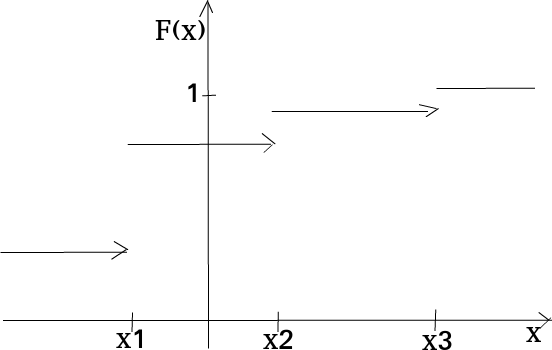
\includegraphics[width=.4\textwidth]{./pictures/9_3.png}
  \caption{Непрерывность справа функции распределения случайной величины}
  \label{fig:93}
\end{figure}

Рассмотрим $P \left( \xi \geq x \right)$.
Перейдём к противоположному
$$P \left( \xi \geq x \right) =
1 - P \left( \xi < x \right) =
1 - \lim \limits_{y \to x-} F \left( y \right).$$
Рассмотрим $P \left( \xi = x \right) $ --- величина скачка в точке.
$$P \left( \xi = x \right) =
P \left( \xi \leq x \right) - P \left( \xi < x \right) =
F \left( x \right) - \lim \limits_{y \to x-} F \left( y \right).$$

Из рисунка \ref{fig:931}
$$P \left( \xi \in \left[ a, b \right] \right) =
P \left( \xi \leq b \right) - P \left( \xi < a \right) =
F \left( b \right) - \lim \limits_{y \to a-} F \left( y \right) =
F \left( b \right) - F \left( a- \right).$$

\begin{figure}[h!]
  \centering
  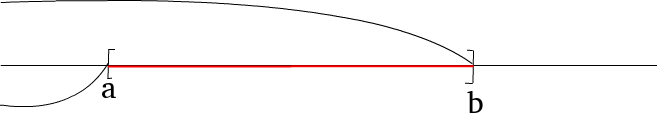
\includegraphics[width=.4\textwidth]{./pictures/9_3_1.png}
  \caption{Отрезок $ \left[ a, b \right] $}
  \label{fig:931}
\end{figure}

\begin{equation*}
\begin{split}
P \left( \left| \xi \right| < x \right) =
P \left( \xi < x \right) - P \left( \xi \leq - x \right) =
\lim \limits_{y \to x-} F \left( y \right) - F \left( -x \right) = \\
= F \left( x- \right) - F \left( -x \right);
\end{split}
\end{equation*}
\item  по определению $F_{- \xi} \left( x \right) = P \left( - \xi \leq x \right) $.
Воспользовавшись непревывностью относительно $ \xi $ получим $P \left( - \xi \leq x \right) = P \left( \xi \geq -x \right) $.
Перейдём к противоположному $P \left( \xi \geq -x \right) = 1 - P \left( \xi < -x \right) = 1 - F_{ \xi } \left( -x- \right) $.

По определению $F_{a \xi + b} \left( x \right) = P \left( a \xi + b \leq x \right) $.
Решаем относительно $ \xi $.
Получаем
$$P \left( a \xi + b \leq x \right) =
P \left( \xi \leq \frac{x-b}{a} \right) =
F \left( \frac{x-b}{a} \right),$$
если $a > 0$.

Пусть $a < 0$.
Тогда будет
$$P \left( \xi \geq \frac{x-b}{a} \right) =
1 - F_{ \xi } \left( \frac{x-b}{a} - \right).$$

Рассмотрим
$$F_{\left| \xi \right| } \left( x \right) =
P \left( \left| \xi \right| \leq x \right) =
P \left( \xi \leq x \right) - P \left( \xi < -x \right) =
F_{ \xi } \left( x \right) - F_{ \xi } \left( -x- \right).$$

Рассмотрим
\begin{equation*}
\begin{split}
F_{ \xi^2} \left( x \right) =
P \left( \xi^2 \leq x \right) =
\begin{cases}
0, \qquad x < 0, \\
P \left| \xi \right| \leq \sqrt{x}, \qquad x \geq 0
\end{cases} = \\
=
\begin{cases}
0, \qquad x < 0, \\
F_{ \xi } \left( \sqrt{x} \right) - F_{ \xi } \left( - \sqrt{x}- \right), \qquad x \geq 0.
\end{cases}
\end{split}
\end{equation*}

Рассмотрим $F_{g \left( \xi \right) } \left( x \right) = P \left( g \left( \xi \right) \leq x \right) $.

Функция $g \left( \xi \right) $ будет случайной величиной, потому что она непрерывна

$$P \left( g \left( \xi \right) \leq x \right) =
\begin{cases}
g \uparrow, \qquad P \left( \xi \leq g^{-1} \left( x \right) \right) = F_{ \xi } \left( g^{-1} \left( x \right) \right), \\
g \downarrow, \qquad P \left( \xi \geq g^{-1} \left( x \right) \right) = 1 - F_{ \xi } \left( g^{-1} \left( x \right) - \right).
\end{cases}$$
\end{enumerate}

\subsubsection*{9.4}

\textit{Задание.} Определите, какие из следующих функций являются функциями распределения:
\begin{enumerate}[label=\alph*)]
\item $F \left( x \right) = 3/4 + 1/ \left( 2 \pi \right) \cdot arctg x $;
\item $F \left( x \right) =
\begin{cases}
0, \qquad x < 0, \\
\frac{x}{1+x}, \qquad x \geq 0;
\end{cases}$
\item $F \left( x \right) =
\begin{cases}
0, \qquad x < 0, \\
\frac{ \left[ x \right] }{2}, \qquad 0 \leq x \leq 2, \\
1, \qquad x > 2.
\end{cases}$
\end{enumerate}

\textit{Решение.}
\begin{enumerate}[label=\alph*)]
\item $F \left( x \right) = 3/4 + 1/ \left( 2 \pi \right) \cdot arctg x $.

Функция
$$arctg x \in \left( - \frac{ \pi }{2}, \frac{ \pi }{2} \right).$$

Подставляя эти значения, получаем
$$ \left( \frac{1}{4}, 1 \right) \in \left[ 0, 1 \right].$$

Проверим следующее свойство
$$ \lim \limits_{n \to + \infty } F \left( x \right) = 1, \,
\lim \limits_{n \to - \infty } F \left( x \right) =
\frac{3}{4} - \frac{1}{4} =
\frac{1}{2} \neq
0.$$

Вывод: это не является функцией распределения;
\item $F \left( x \right) =
\begin{cases}
0, \qquad x < 0, \\
\frac{x}{1+x}, \qquad x \geq 0.
\end{cases}$

Функция непрерывна, $0 \leq F \left( x \right) \leq 1$.

Найдём значение функции на бесконечности
$$F \left( - \infty \right) =
\lim \limits_{x \to - \infty } F \left( x \right) =
0, \,
F \left( + \infty \right) =
\lim \limits_{x \to + \infty } F \left( x \right) =
1.$$

При $x \geq 0$ берём рпоизводную
$$F' \left( x \right) =
\left( \frac{x}{1+x} \right)' =
\frac{1+x-x}{ \left( 1+x \right)^2} =
\frac{1}{ \left( 1+x \right)^2} >
0.$$

Берём вторую производную
$$F'' \left( x \right) =
\frac{-2 \left( x+1 \right) }{ \left( 1+x \right)^4} <
0.$$
Отсюда следует, что функция выпуклая вверх (рис. \ref{fig:94});

\begin{figure}[h!]
  \centering
  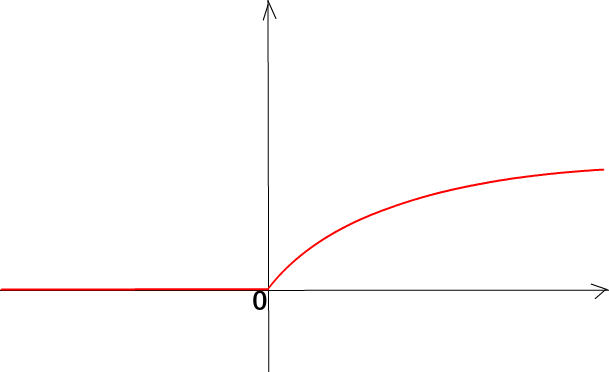
\includegraphics[width=.4\textwidth]{./pictures/9_4.png}
  \caption{Вид функции распределения}
  \label{fig:94}
\end{figure}

\item $F \left( x \right) =
\begin{cases}
0, \qquad x < 0, \\
\frac{ \left[ x \right] }{2}, \qquad 0 \leq x \leq 2, \\
1, \qquad x > 2.
\end{cases}$

По графику (рис. \ref{fig:941}) это является функцией распределения.

\begin{figure}[h!]
  \centering
  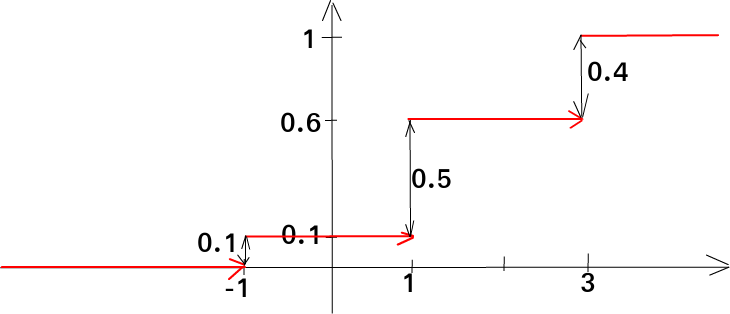
\includegraphics[width=.4\textwidth]{./pictures/9_4_1.png}
  \caption{График функции распределения}
  \label{fig:941}
\end{figure}

\end{enumerate}

\subsubsection*{9.5}

\textit{Задание.} Постройте график функции распределения случайной величины $ \xi $ такой, что
$P \left( \xi = 1 \right) = 0.5, \,
P \left( \xi = 3 \right) = 0.4, \,
P \left( \xi = -1 \right) = 0.1$.

\textit{Решение.} В сумме вероятности дают единицу, значит это все значения, которые может принимать $ \xi $.
По определению
$$F \left( x \right) =
P \left( \xi \leq x \right) =
\begin{cases}
0, \qquad x < -1, \\
0.1, \qquad -1 \leq x < 1, \\
0.6, \qquad 1 \leq x < 3, \\
1, \qquad x \geq 3.
\end{cases}$$

Найдём $P \left( \xi \leq 2 \right) = P \left( \xi = 1 \right) + P \left( \xi = -1 \right) $.

График имеет вид как на рисунке \ref{fig:95}.

\begin{figure}[h!]
  \centering
  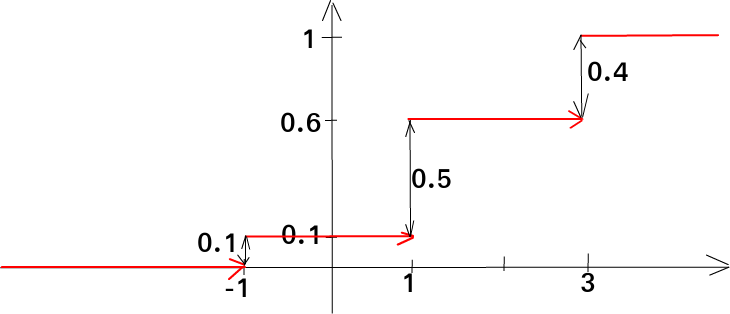
\includegraphics[width=.4\textwidth]{./pictures/9_5.png}
  \caption{Вид функции распределения}
  \label{fig:95}
\end{figure}

Вероятности --- величина скачка.

\addcontentsline{toc}{section}{Дополнительные задачи}
\section*{Дополнительные задачи}

\addcontentsline{toc}{section}{Домашнее задание}
\section*{Домашнее задание}
